\documentclass[10pt,a4paper]{scrartcl}
\usepackage[utf8]{inputenc}
\usepackage{ngerman}
\usepackage{graphicx}
\usepackage[final]{listings}
\lstset{tabsize=2,basicstyle=\ttfamily\small}
\usepackage[draft]{fixme}
\usepackage{color}
\definecolor{LinkColor}{rgb}{0.0,0.0,0.0} 
\usepackage[
        bookmarks=true,
        bookmarksopen=true,
        bookmarksopenlevel={1},
        bookmarksnumbered=true,
        plainpages=false,
        pdfpagelabels=true,
        hypertexnames=false,
        pdftitle={},
        pdfauthor={Sven Wenzel},
        pdfcreator={LaTeX with hyperref and KOMA-Script},
        pdfsubject={},
        pdfkeywords={},
        final]{hyperref}
\hypersetup{colorlinks=true,
        anchorcolor=LinkColor,
        linkcolor=LinkColor,
        citecolor=LinkColor,
        filecolor=LinkColor,
        menucolor=LinkColor,
        pagecolor=LinkColor,
        urlcolor=LinkColor}

\newcommand{\hinweis}[1]{

\textbf{Hinweis:} #1

}

\newcommand{\review}[1]{
	\hfil\\
	\textbf{\textcolor{red}{#1}}
	\hfil\\
}

\title{Introduction to the SiDiff 2.0 Development Environment}
\author{Timo Kehrer}
\begin{document}
\maketitle
\tableofcontents
\newpage
\section*{Dokumenthistorie}
Dieses Dokument wird fortlaufend gepflegt. Die nachfolgende Tabelle gibt 
eine Übersicht über die Änderungen in einzelnen Versionen.

\begin{tabular}{|c|p{11cm}|}\hline
Datum & Änderungen \\\hline\hline
16.09.09 & erste Version \\\hline
\end{tabular} 


\newpage

\section{Erstellen und Starten einer Laufzeitumgebung}
Das Einrichten einer Laufzeitumgebung erfolgt in Eclipse
mittels \emph{Run $\to$ Run configurations ...}. Der Dialog zeigt bestehende 
Laufzeitumgebungen und ermöglicht diese zu konfigurieren. Wir richten hier eine 
neue ein.

Hierzu ist links \emph{OSGi Framework} auszuwählen und der \emph{New}-Button (oben)
zu klicken. Eine neue Laufzeitumgebung wird angelegt. Im rechten Teil des Fensters
kann die Umgebung konfiguriert werden.

\begin{center}
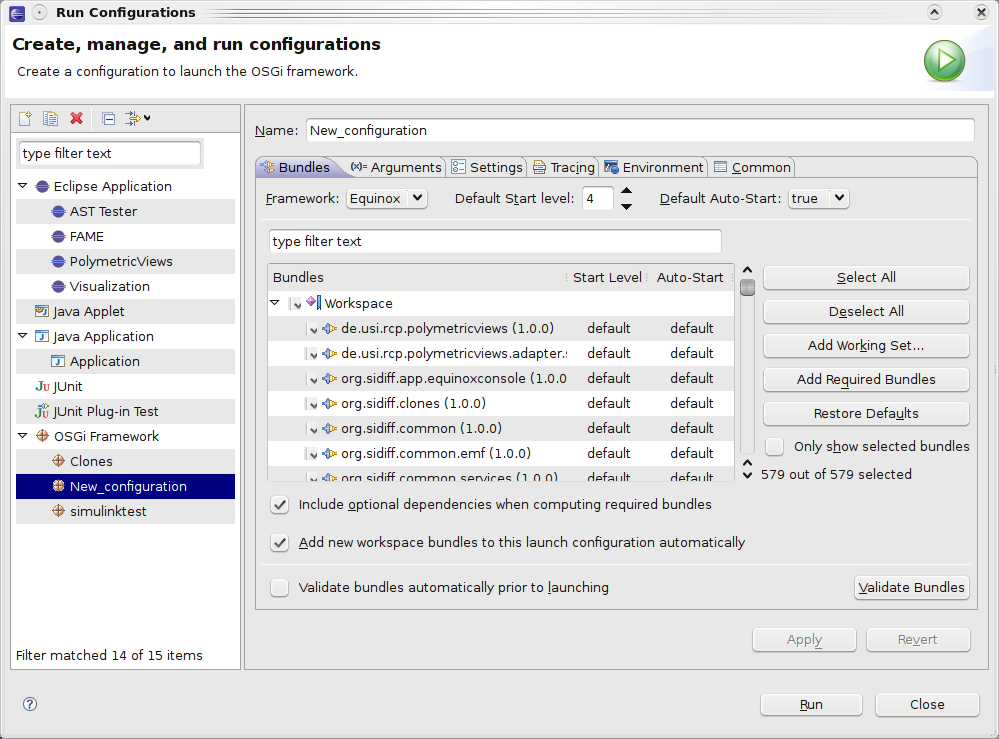
\includegraphics[width=12cm]{pics/runconfig1.png}
\end{center}

Unter \emph{Bundles} können die Bundles ausgewählt werden, die man in der
Laufzeitumgebung haben möchte. Hier können auch Eclipse-Plugins ausgewählt werden, 
weil diese prinzipiell auch OSGi-Bundles sind. 
\hinweis{Um zu verhindern, dass man letzlich wieder ein komplettes Eclipse startet
sollte man:
\begin{enumerate}
 \item Target-Platform deselektieren (alle untergeordneten Bundles werden automatisch
deselektiert)
 \item Mit dem Button \emph{Add Required Bundles} werden alle notwendigen Bundles (z.B.
für Dateizugriff) wieder ausgewählt.
\end{enumerate}
}

Unter \emph{Arguments} können Parameter für das OSGi-Framework und die Virtual Machine (VM)
gesetzt werden. Die OSGi-Parameter sollten nicht verändert werden. Die VM-Parameter können
nach belieben erweitert werden, z.b. um mit \texttt{-Xmx512m} mehr Arbeitsspeicher bereitzustellen.

\hinweis{Konsolenapplikation können durch die Kombination des Arguments \texttt{-console} und
des VM-Parameters \texttt{-Dosgi.noShutdown=true} realisiert werden.}


Die übrigen Konfigurations-Tabs werden für unsere Zwecke nicht benötigt.

\review{TODO: Auch andere Tabs können von Bedeutung sein, so z.B. für das Anlegen von *.launch-Dateien.
Auch weitere Konfigurationsmöglichkeiten wie das Workind-Directory lohnt es sich im Rahmen
eines neuen WhitePapers evtl. zu beschreiben.}


\subsection{Starten der Laufzeitumgebung}
Die Laufzeitumgebung wird einfach mit \emph{Run} gestartet. Nach wenigen Sekunden steht uns
im \emph{Colsole}-View von Eclipse die OSGi-Konsole zur Verfügung. Hier ein paar nützliche
Kommandos:
\begin{itemize}
 \item \texttt{ss} gibt eine Übersicht (short status) über vorhandene Bundles aus. Die Liste 
sollte zwischen 50 und 100 Bundles betragen, jenachdem welche Bundles ausgewählt wurden. Werden
500 oder mehr Bundles gelistet, ist dies ein Indiz für eine vollständige Eclipse-Instanz.
Die Liste gibt außerdem an, in welchem Zustand ein Service ist. (siehe Service-Status)
 \item \texttt{start XX} aktiviert den Service mit der Nummer XX (aus der Liste). Bei diesem 
manuellen Start werden auch ggf. vorhandene Exceptions ausgegeben, die beim automatischen 
Startversuch nicht anzegeigt werden.
 \item \texttt{stop XX} deaktiviert den Service mit der Nummer XX. \\[0.5cm]\texttt{start} 
und \texttt{stop} können genutzt werden, um abwechselnd verschiedene Service-Implementierungen
einzusetzen.
\end{itemize}

\paragraph{Service-Status}
Der Lebenszyklus eines OSGi-Bundles sieht folgende Zustände vor:
\begin{center}
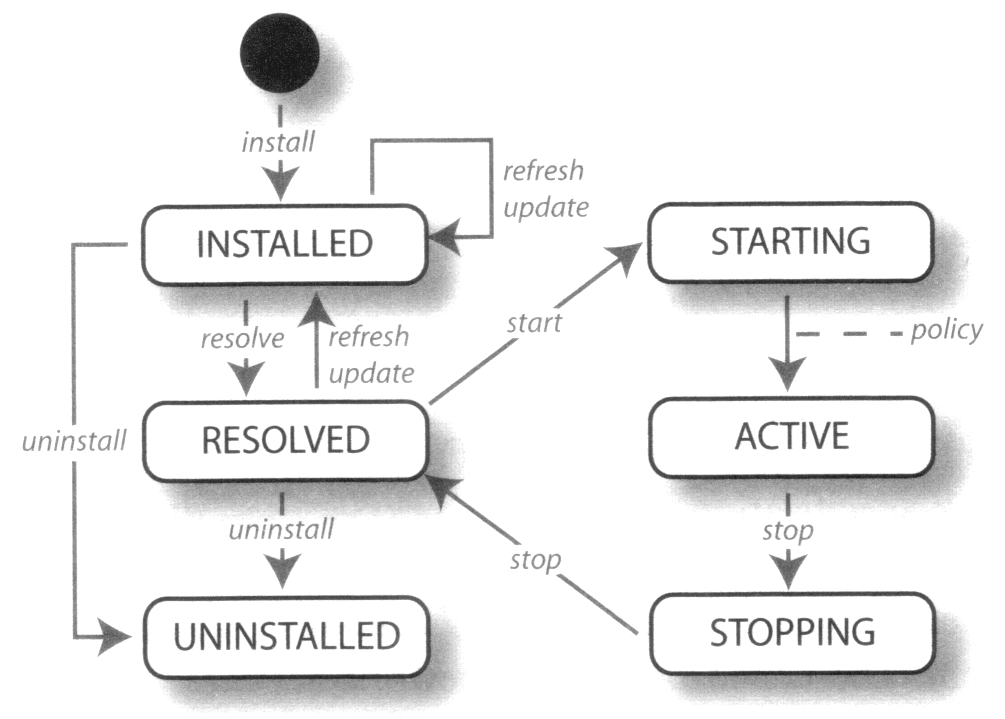
\includegraphics[width=8cm]{pics/osgilifecycle.png}
\end{center}
Bundles sind zunächst \emph{installiert}, d.h. sie stehen dem System zur Verfügung, wenn wir
sie der Laufzeitumgebung hinzufügen. Das OSGi-Framework prüft sofort nach der Installation,
ob alle Voraussetzungen erfüllt sind, damit das Bundle ``einsatzfähig'' ist. Ist dies der Fall
wechselt das Bundle in den Zustand \emph{resolved}. Hier kann das Bundle mit \texttt{start} 
und \texttt{stop} aktiviert bzw. deaktiviert werden. Ist der Start nicht möglich (z.B. aufgrund
einer Exception), bleibt das Bundle \emph{resolved}. Bei erfolgreichem Start wird es \emph{active}.
\emph{Starting} und \emph{Stopping} beschreiben die Zeitspanne der (De-)Aktivierung. 

(Für Fortgeschrittene: Sie entsprechen den Methoden im Activator.)


\clearpage
\section{Kochrezept A: Erstellen eines Bundles, das Klassen und Ressourcen bereitstellt}
\review{Inhalt des Kapitels wurde noch nicht reviewed}

\paragraph{Schritt 1:}
\begin{center}
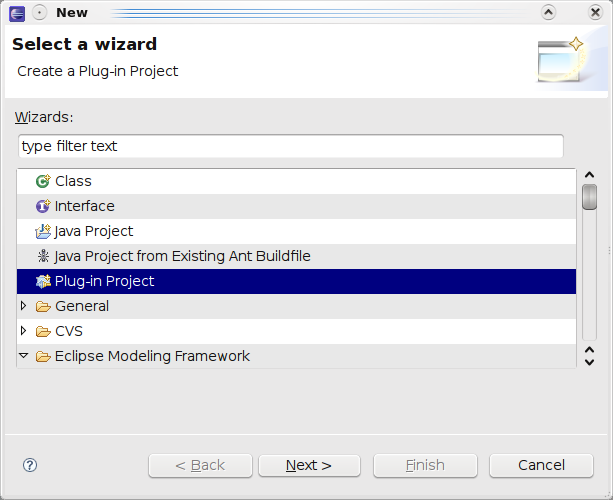
\includegraphics[width=7cm]{pics/newbundle1.png}
\end{center}
Erstelle ein neues Plugin-Projekt mit dem Eclipse-Wizard.

\paragraph{Schritt 2:}
\begin{center}
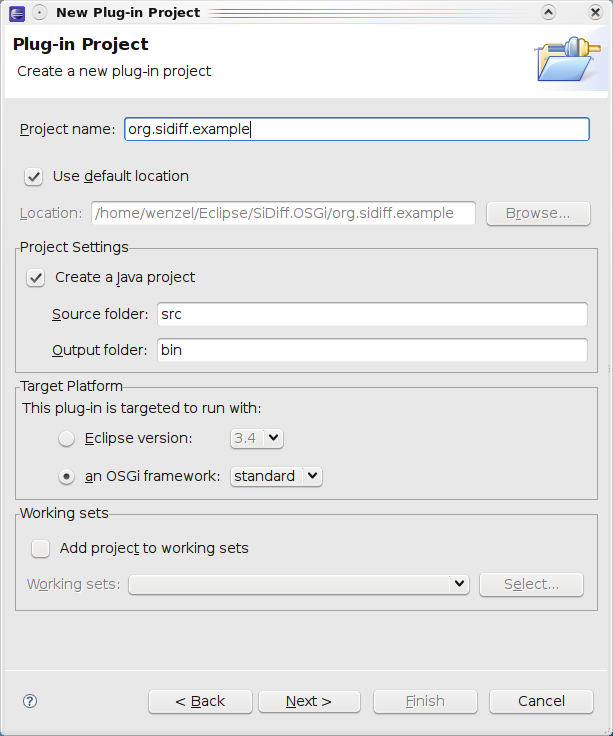
\includegraphics[width=8cm]{pics/newbundle2.png}
\end{center}
Wähle den Bundlenamen gemäß Konvention und setze ihn als Projektnamen. Bei den
Project Settings wähle \emph{Create a Java Project} aus und definiere \emph{src}
als Source folder und \emph{bin} als Output folder. Als Target Platform ist
\emph{an OSGi framework} zu wählen. Achtung: Hier muss in der Dropdown-Box noch
\emph{standard} ausgewählt werden.

\paragraph{Schritt 3:}
\begin{center}
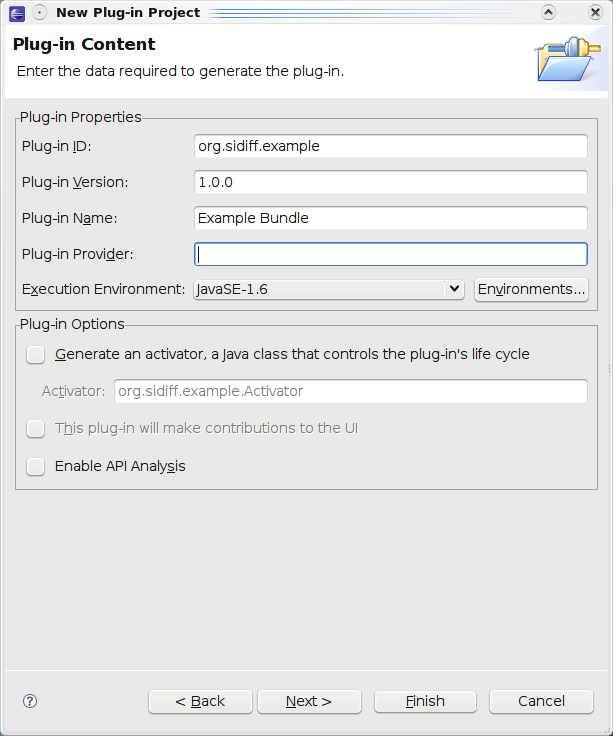
\includegraphics[width=8cm]{pics/newbundle3.png}
\end{center}
Im nächsten Dialog sollte bei Plugin-ID der Bundlename stehen. Ist dies nicht
der Fall, so ist nochmal einen Schritt zurückzugehen und der Projektname neu zu
setzen. Die Version sollte defaultmäßig bei 1.0.0 bleiben. Der Plugin-Name ist
frei wählbar, ebenso der Plugin-Provider\footnote{Hierfür wird es später mal ein
geeignetes Template geben.}. Als Execution-Environment ist Java 1.6 auszuwählen.

Bei Plugin-Options kann man noch auswählen, ob ein Activator erstellt werden soll.
Ein Activator ermöglicht die Ausführung von Code, wenn ein Bundle innerhalb des
OSGi-Frameworks aktiviert wird (d.h. i.d.R. bei erstmaligem Zugriff). Zur 
Bereitstellung von Klassen und Ressourcen ist das i.d.R. nicht nötig.

Sollte dieser Schritt vergessen worden sein, kann auch nachträglich ein Activator 
angelegt werden. 
Hierzu klickt man in der Übersicht des Manifest-Editors (siehe Schritt 4) auf
das unterstrichene Label ``Activator''. Mithilfe des erscheinenden Dialogs kann
der Activator angelegt werden. Wie der Activator konkret zu implementieren ist,
wird später gezeigt.

\paragraph{Schritt 4:}
\begin{center}
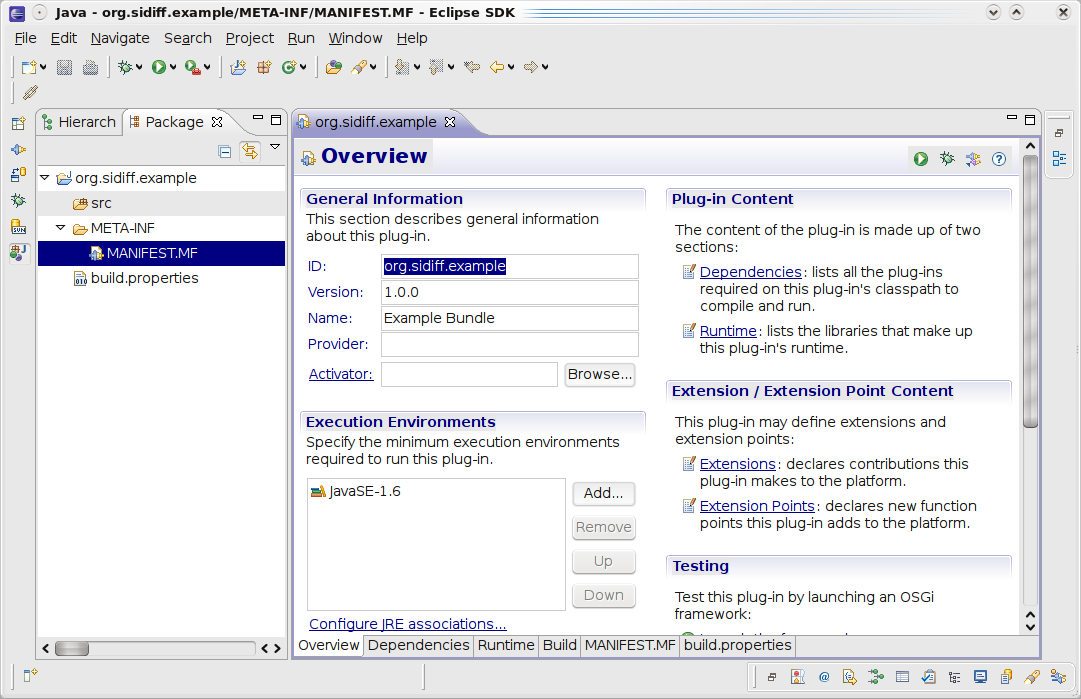
\includegraphics[width=12cm]{pics/newbundle4.png}
\end{center}
Der Manifest-Editor zeigt nun eine Übersicht über das neue Bundle. Hier können
später Äbhängigkeiten zu anderen Bundles, Freigaben und Build-Eigenschaften
eingestellt werden (siehe Tabs am unteren Rand).

\paragraph{Schritt 5:}
\begin{center}
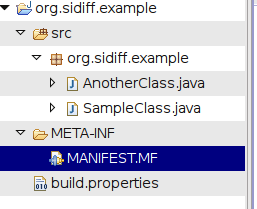
\includegraphics[width=5cm]{pics/newbundle5.png}
\end{center}
Zunächst muss das Basis-Paket angelegt werden. Es heißt wie das Bundle. Darin
können nach Belieben Klassen und weitere Pakete angelegt werden.

\paragraph{Schritt 6:}
Implementierung der Klassen

\paragraph{Schritt 7:}
\begin{center}
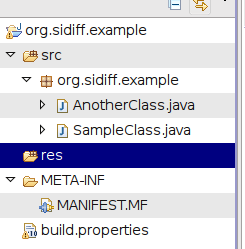
\includegraphics[width=5cm]{pics/newbundle6.png}
\end{center}
Sollen neben Java-Code auch Ressourcen, z.B. Bilder, XML-Dateien oder sonstiges
bereitgestellt werden, so können weitere Source-Ordner angelegt werden. Dateien
dieser Ordner landen später automatisch im Jar-Archiv eines Bundles.

\paragraph{Schritt 8:}
\begin{center}
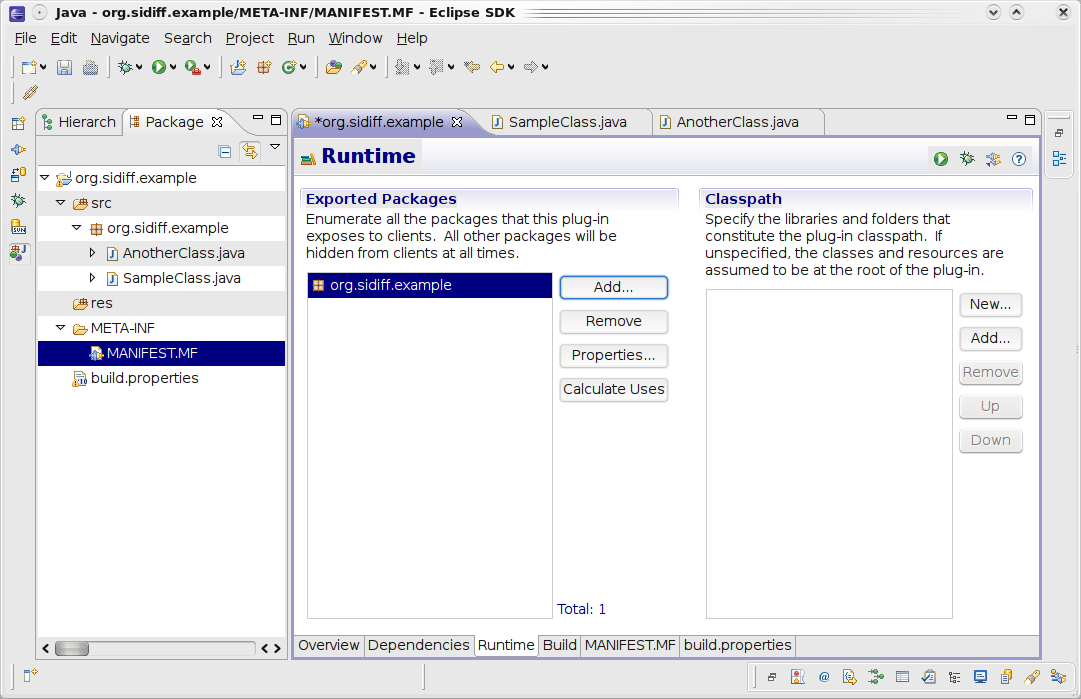
\includegraphics[width=12cm]{pics/newbundle7.png}
\end{center}
Damit die Java-Klassen von anderen Bundles genutzt werden können, müssen diese
explizit freigegeben werden. Dieses geschieht über den Tab ``Runtime'' des
Manifest-Editors. Bei \emph{Exported Packages} sind diejenigen Pakete auszuwählen,
die nach aussen freigegeben werden sollen.

Falls Abhängigkeiten zu anderen Bundles bestehen, können diese unter dem Tab
\emph{Dependencies} eingetragen werden.

\paragraph{Benutzen des Bundles:}
Die Klassen und Ressourcen des neuen Bundles können nun einfach in anderen
Bundles benutzt werden. Hierzu ist einfach eine Abhängigkeit zu unserem neu
erstellten Bundle einzutragen.



\clearpage
\section{Häufige Stolperfallen}

Wenn mal etwas nicht läuft wie es soll, kann oft eine der nachfolgenden
Stolperfallen ein Grund dafür sein:

\subsection{Beim Kompilieren}

\paragraph{Abhängigkeiten zwischen Bundles} Sind alle benötigten Bundles im
Manifest-Editorals ``Required Plugins'' in den \emph{Dependencies} eingetragen?

\paragraph{Freigabe von Paketen} Sind alle Pakete, die in anderen Bundles zur
Verfügung stehen sollen im Manifest-Editor unter \emph{Runtime} als ``Exported
Packages'' angegeben?

\subsection{Zur Laufzeit}
\paragraph{Activator wird nicht ausgeführt} Oftmals wird der Activator nicht 
ausgeführt weil schlichtweg vergessen wurde, ihn in der MANIFEST.MF einzutragen.
Ein weiteres Problem besteht, wenn der Namespace nicht eindeutig ist. Hierzu 
empfehle ich, den Activator immer in ein Paket mit dem Namen des Bundles 
abzulegen.

\paragraph{Ladereihenfolge von Bundles / Exceptions im Activator} Bundles können
in unterschiedlichster Reihenfolge beim OSGi-Framework registriert werden.
Explizite Abhängigkeiten werden zwar i.d.R. durch das Framework aufgelöst,
jedoch erfolgt diese Auflösung erst im Zuge der Aktivierung der Bundles. Deshalb
sollte man vermeiden, im Activator bereits die Aktivierung anderer Bundles
vorauszusetzen.

Wenn andere Bundles zwingend notwendig sind kann man mit Hilfe eines Listeners
auf die Aktivierung der Bundles warten:
\begin{lstlisting}
public class Activator implements BundleActivator {
	BundleContext context;
	BundleListener listener = new BundleListener() {
		@Override
		public void bundleChanged(BundleEvent event) {
			if (event.getType() == BundleEvent.STARTED ||
			 org.sidiff.example.myservice.Activator.BUNDLE_NAME.equals(
			 event.getBundle().getSymbolicName())) {
				OtherService os = ServiceHelper.getService(context, OtherService.class);
				if (os != null) {
					os.doSomethingElse();
					context.removeBundleListener(listener);
				}
			}
		}
	};
	
	public void start(BundleContext context) throws Exception {
		this.context = context;
		context.addBundleListener(listener);
	}

	public void stop(BundleContext context) throws Exception {
		context.removeBundleListener(listener);
	}

\end{lstlisting}

\paragraph{Klassen aus anderen Bundles lassen sich nicht per Reflection laden}
Der OSGi-Standard sieht vor, dass jedes Bundle seinen eigenen ClassLoader
zugeteilt bekommt, damit sich verschiedene Bundles nicht gegenseitig stören
können. Dieses Prinzip behindert die Idee, mit einem Bundle Klassen
bereitzustellen, die an anderer Stelle reflektiv (also mit einem anderen
ClassLoader) geladen werden sollen. 

Das Problem kann umgangen werden, indem das Bundle, das die Klassen anbietet,
seinen ClassLoader dem \texttt{ResourceUtil} aus dem Bundle
\texttt{org.sidiff.common} bekannt macht: 
\begin{lstlisting}
ResourceUtil.registerClassLoader(this.getClass().getClassLoader());
\end{lstlisting}
Anschließend können die alle Klassen dieses Bundles mit Hilfe des
\texttt{ReflectionUtil} (ebenfalls aus \texttt{org.sidiff.common}) reflektiv
geladen werden.


\end{document}
